\section{Methods}\label{sec:methods}
\subsection{Isolated Setup}\label{ssec:iso_setup}
We use a modified version of the \texttt{MakeNewDisk} variant described in \citet{2023MNRAS.tmp.2070B}. In isolation, each of the central and satellite galaxies are a compound halo setup, with a \citet{1990ApJ...356..359H} dark matter halo and a gaseous halo with a $\beta$-profile:
\begin{equation*}
\rho = \rho_0 \left[1 + \left(\frac{r}{r_c}\right)^2\right]^{-\frac{3\beta}{2}}
\end{equation*}
The total mass within the virial radius is kept fixed, and the mass of the dark matter halo and central density of the gaseous halo are chosen to satisfy a given baryon fraction $f_b$. The dark matter halo is initialized to be in gravitational equilibrium with the total potential. The gaseous halo is in gravito-hydrostatic equilibrium, where the temperature is allowed to vary as a function of radius. The azimuthal velocity of the gaseous halo is given as a fraction of the circular velocity. There is no initial stellar disk or bulge, and the gas is initially metal-free. Thus, all star particles and metals are formed self-consistently.

We used the fiducial halos in \citet{2021ApJ...923...92N} as a starting point for each galaxy. We then manually varied the different model parameters until we arrived at a setup that resulted in reasonable galaxies as determined by their stellar mass. For the central (Milky Way) galaxy, we set $M_{200}=5\times10^{11}\,\Msun$, $c_{200}=4.1$, $\beta=0.8$, $r_c=9\,\kpc$, $f_b=0.08$, and $v_{\phi}/v_{\textrm{c}}=0.2$, where $c_{200}$ is the concentration and $v_{\phi}/v_{\textrm{c}}$ is the azimuthal velocity of the gaseous halo as a fraction of the local circular velocity. For the satellite (GSE) galaxy, we set $M_{200}=2.2\times10^{11}\,\Msun$, $c_{200}=4.33$, $\beta=0.8$, $r_c=6.5\,\kpc$, $f_b=0.06$, and $v_{\phi}/v_{\textrm{c}}=0.4$.

We used a mass resolution of $6\times10^4\,\Msun$ for the gas and $3\times10^5\,\Msun$ for the dark matter. This is closest to a resolution of level 4 in the AURIGA simulations \citep{2017MNRAS.467..179G}, and is about $0.7\times$ the mass resolution of TNG50-1 \citep{2019MNRAS.490.3234N,2019MNRAS.490.3196P}. All collisionless particles have a fixed softening length of $40\,\pc$. The gas has a softening length $2.5\times$ the cell size, with a minimum size of $10\,\pc$. Snapshots were saved at intervals of $25\,\Myr$.

The stellar mass build-up of our Milky Way-like and GSE-like galaxies is given in Figure~\ref{fig:mass_size}. The upper panel shows the stellar mass history. We attempt to match the expected mass of the present-day thick disk \citep[$\sim6\times10^9\,\Msun$, horizontal blue dashed line][]{2016ARA&A..54..529B} at an evolution time of $\sim3\,\Gyr$ (corresponding to $z\sim2$, vertical dashed gray line).\footnote{Of course, this neglects the significant mass contribution of the bulge, which presumably formed earlier. However, our setup does not form a strong spheroidal component. Using the trick in e.g. \citet{2022MNRAS.515.1524Z}, we take the bulge mass to be twice the counterrotating stellar mass. At $3\,\Gyr$ in the isolated Milky Way-like galaxy, the bulge mass is $\sim7\times10^{8}\,\Msun$, or $\sim13\%$ of the total mass. The Milky Way's bulge is  $\sim1.5\times10^{10}\,\Msun$, although there is strong debate about just how much of the bulge is a classical bulge which formed before the disk \citep{2016ARA&A..54..529B}. In any case, we did not attempt to match any particular property of the bulge, though one could promote bulge formation by reducing the rotation of the gas in the inner region.} We get reasonably close at $\sim5\times10^9\,\Msun$ (blue line). For GSE, we use the best-fit mass from the $N$-body simulations of \citet{2021ApJ...923...92N} -- $5\times10^8\,\Msun$ (horizontal dashed orange line). For this, we slightly overestimate at $\sim6\times10^8\,\Msun$ (orange line).

As for the galaxy sizes, there is significant spread amongst the real galaxy population, and the sizes are thought to be influenced by the merger history not present in our setup \citep[e.g.][]{2014ApJ...788...28V}. We note that the sizes of each simulated galaxy (lower panel) are within the range of observed galaxy sizes. For the Milky Way, we know the thick disk has scale length of $\sim2\,\kpc$, which converts to a half-mass radius of $\sim3.36\,\kpc$. At $\sim3\,\Gyr$, our Milky Way-like galaxy has a half-mass radius of $\sim2\,\kpc$. Curiously, after $3\,\Gyr$, the size of the Milky Way-like galaxy continues to grow while the GSE galaxy's size remains constant for the duration of the simulation.

\begin{figure}
    \centering
    \includegraphics[width=\columnwidth]{mass_size.pdf}
    \caption{The mass and size evolution of the central (Milky Way, blue) and satellite (GSE, orange) galaxies. The mass is taken to be the stellar mass within twice the half-mass radius, and the size is taken to be the half-mass radius. In the upper panel, we also show as a horizontal line the mass of the Milky Way's disk and GSE from the best-fit model of \citet{2021ApJ...923...92N}. This comparison is taken to be made at $3\,\Gyr$ (vertical dashed line), our proxy for $z\sim2$. A precise match is not attempted given the wide ranging uncertainties.}
    \label{fig:mass_size}
  \end{figure}

\subsection{Orbital Configuration}\label{ssec:orbit_setup}
In order to combine the galaxies, we follow \citet{2021ApJ...923...92N}, and place the satellite on a retrograde orbit. In the fiducial simulation of \citet{2021ApJ...923...92N}, the satellite is placed at the virial radius ($129\,\kpc$), with the virial velocity ($129\,\kms$), and with a circularity of $0.5$. To test minor changes to the orbit, we ran a grid of simulations with $\pm10\%$ in each the starting radius and velocity, and $\pm0.1$ in the circularity, for a total of $27$ simulations. We performed each simulation for a duration of $8\,\Gyr$, and used \texttt{FOF} and \texttt{SUBFIND} in order to identify substructure \citep{2005Natur.435..629S,2009MNRAS.399..497D}.

Some of the simulations in this orbital grid resulted in bimodal abundance distributions, while some had little to no structure in the abundance distribution plane. We show the abundance plane for all $27$ simulations in Appendix~\ref{app:allmerge}, but for the main body of this work we consider two representative simulations in detail which were chosen based on their structure in the abundance plane as shown in Figure~\ref{fig:fig1}. For the bimodal simulation, we chose the simulation with $R_0=142\,\kpc$, $V_0=116\,\kms$, and $\eta=0.4$. For the unimodal simulation, the parameters are the same except that $R_0=129\,\kpc$.

We show the bimodal and unimodal simulations' orbits in Figure~\ref{fig:orbit}. For the center of the central and satellite, we use the position of the particle with minimum potential in each substructure identified by \texttt{SUBFIND}. The upper and middle panels show the orbits in the $x$-$y$ and $x$-$z$ planes, respectively. The lower panel shows the separation distance as a function of time. The orbit is initially retrograde, but quickly radializes after the first pericentric passage. Coalescence occurs rapidly after the second pericentric passage at $\sim2\,\Gyr$, and \texttt{SUBFIND} ceases to recognize the satellite as a separate subhalo.

\begin{figure}
    \centering
    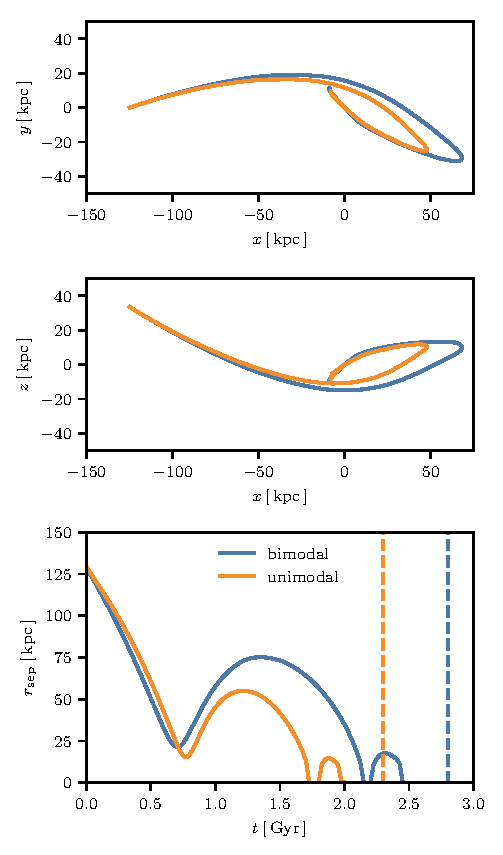
\includegraphics[width=\columnwidth]{orbit.pdf}
    \caption{The orbits of the bimodal (blue) and unimodal (orange) simulations. The upper and middle panels show the orbit in the $x$-$y$ and $x$-$z$ planes, respectively. The bottom panel shows the separation distance as a function of time. The orbit begins retrograde but then radializes after the first pericentric passage. The satellite then coalesces quickly after the second pericentric passage, after $\sim2\,\Gyr$ of evolution.}
    \label{fig:orbit}
\end{figure}

\subsection{Feedback and Enrichment Model}\label{ssec:gfm}
Our feedback model is most closely related to that used in the Illustris TNG simulation suite \citep{2013MNRAS.436.3031V,2017MNRAS.465.3291W,2018MNRAS.473.4077P}. In this model, gravity and magnetohydrodynamics are solved using a \citet{1986Natur.324..446B} tree coupled to a second order finite volume fluid solver in AREPO \citep{2010MNRAS.401..791S,2016MNRAS.455.1134P}. Stellar feedback is included through a subgrid wind particle model \citep{2003MNRAS.339..289S}. AGN feedback follows a dual kinetic and thermal mode for low- and high-accretion rates \citep{2017MNRAS.465.3291W}, though in our setup the AGN is only ever in the high-accretion mode. The central galaxy is seeded with a black hole with the typical seed mass ($8\times10^5\,\Msun$). 

In this work, we made some simplifications to this model in order to aid interpretation. First, we ignore magnetic fields. This was motivated by an initial desire to understand the CGM accretion rates in terms of idealized cooling flow solutions, but we did not revisit turning them back on. In any case, it is not clear if the magnetic fields would be realistically generated given our initial setup. Second, we use a gentler wind feedback model as described in \citet{2019MNRAS.489.4233M}. Because our setup includes both an initially steep central potential and no steady-state disk, a stronger feedback model would require a higher central gas density to achieve a reasonable SFH which introduced its own set of pathological instabilities.

In this model, star particles synthesize elements through three different channels for which we cite the relevant yield tables: SNe Ia \citep{1997NuPhA.621..467N}, SNe II \citep{1998A&A...334..505P,2006ApJ...653.1145K}, and AGB stars \citep{2010MNRAS.403.1413K,2014MNRAS.437..195D,2014ApJ...797...44F}. Recall that star particles are simple stellar populations (i.e., a collection of stars with the same age and chemical composition). Each star particle continuously injects metals into its surroundings in the following sequence\footnote{The kinetic/thermal feedback component is handled through the wind generation, which is completely separate in this model.}:
\begin{enumerate}
    \item $t\lesssim10\,\Myr$: no metal injection as the first supernova ($M\sim100\,\Msun$) has not gone off
    \item $10\,\Myr \lesssim t \lesssim 40\,\Myr$: metal injection as $8\,\Msun<M<100\,\Msun$ stars die as Type II SNe
    \item $t\gtrsim40\,\Myr$: metal injection from Type Ia SNe and AGB stars
\end{enumerate}
There are a few things to note about this model: (1) The exact timings are metallicity-dependent. (2) The \MgFe{} of ejected gas from Type II SNe is mass/time-dependent, with more massive stars contributing more Mg than less massive stars. (3) In a Hubble time, type II SNe contribute the vast majority of Mg ($\sim10\times$ AGB and $\sim100\times$ Type Ia SNe). Type Ia and Type II SNe contribute approximately equal amounts of Fe (each $\sim3\times$ AGB). See Figure~1 from \citet{2018MNRAS.473.4077P}. (4) The number of Type Ia SNe is greater for a younger stellar population, with a power law relationship $\propto \left(t/\tau_8\right)^{-1.12}$, where $\tau_8=40\,\Myr$ is the lifetime of an $8\,\Msun$ star.

\subsection{Observed Abundances}\label{ssec:obs_abund}
Our aim in this work is to demonstrate the feasibility of a mechanism for structure formation in the abundance plane. We are only making a qualitative comparison to data. Therefore, we use the ASPCAP DR17 catalog of stellar abundances \citep[][J.A.~Holtzman et al., in preparation]{2016AJ....151..144G}, which is publicly available, well-established, and widely used.

We first make some quality cuts, as well as restricting our sample to giants. We require:
\begin{itemize}[noitemsep]
    \item $\textrm{SNR} > 200$,
    \item $\textrm{VSCATTER} < 1\,\kms$,
    \item STARFLAG not set,
    \item $\varpi/\sigma_{\varpi} > 1$,
    \item $\log{g} < 3.5$,
    \item $\sigma_{\log{g}} < 0.2$,
\end{itemize}
where $\varpi$ is the parallax. We use the parallax, proper motion, and radial velocity from Gaia EDR3 \citep{2016AA...595A...1G,2021AA...649A...1G,2021AA...649A...2L,2021AA...653A.160S}.

We next make a selection on the angular momentum of stars in order to make a solar neighborhood selection. We assume the solar radius and azimuthal velocity are $R_0=8\,\kpc$ and $V_0=220\,\kms$ \citep{2016ARA&A..54..529B}, and select stars which have $L_z$ within $10\%$ of the solar angular momentum. We further require that $\left|z\right| < 3\,\kpc$.

As is typically done, we use \FeH{} as an indicator of the total metallicity of a star. We use Mg alone as a representative of the $\alpha$-elements.

\subsection{Solar Neighborhood in Simulations}\label{ssec:solarneigh}
When comparing galaxy simulations to the observed solar neighborhood, some ambiguity arises in how to make a ``solar neighborhood-like'' selection of star particles. Naturally, this selection is dependent on the posed question, which in this work is the formation of the abundance bimodality. The Sun is known to sit near the end of the thick disk, where the thick and thin disk have comparable surface densities \citep[the ratio of thick-to-thin is $\sim12\%$][]{2016ARA&A..54..529B}. As a result, the abundance bimodality appears most strongly near the Sun -- further inwards the high-$\alpha$ sequence is more dominant and further outwards the high-$\alpha$ sequence vanishes \citep[e.g.,][]{2015ApJ...808..132H}.

We mimic our selection of the solar neighborhood by also making a cut in angular momentum. However, in the simulation, the high-$\alpha$ disk is more compact than in the Galaxy. Therefore, in order to strike a balance between the low-$\alpha$ and high-$\alpha$ disks, we used an angular momentum cut which is $20\%$ that of our assumed solar angular momentum. In particular, we select all star particles with angular momenta within $30\%$ of $0.2\times8\,\kpc\times220\,\kms$ -- as well as requiring $\left| z \right| < 3\,\kpc$. This corresponds to roughly selecting star particles with radii between $2$ and $5\,\kpc$.
